\documentclass[letterpaper,final,12pt,reqno]{amsart}

\usepackage[total={6.3in,9.2in},top=1.1in,left=1.1in]{geometry}

\usepackage{times,bm,bbm,empheq,verbatim,fancyvrb,graphicx}
\usepackage[dvipsnames]{xcolor}

\usepackage[kw]{pseudo}

\pseudoset{left-margin=15mm,topsep=5mm,idfont=\texttt}

\usepackage{tikz}
\usetikzlibrary{decorations.pathreplacing}

% hyperref should be the last package we load
\usepackage[pdftex,
colorlinks=true,
plainpages=false, % only if colorlinks=true
linkcolor=blue,   % ...
citecolor=Red,    % ...
urlcolor=black    % ...
]{hyperref}

\renewcommand{\baselinestretch}{1.05}

\newtheorem{lemma}{Lemma}

\newcommand{\Matlab}{\textsc{Matlab}\xspace}
\newcommand{\eps}{\epsilon}
\newcommand{\RR}{\mathbb{R}}

\newcommand{\grad}{\nabla}
\newcommand{\Div}{\nabla\cdot}
\newcommand{\trace}{\operatorname{tr}}

\newcommand{\hbn}{\hat{\mathbf{n}}}

\newcommand{\bb}{\mathbf{b}}
\newcommand{\be}{\mathbf{e}}
\newcommand{\bbf}{\mathbf{f}}
\newcommand{\bg}{\mathbf{g}}
\newcommand{\bn}{\mathbf{n}}
\newcommand{\br}{\mathbf{r}}
\newcommand{\bu}{\mathbf{u}}
\newcommand{\bv}{\mathbf{v}}
\newcommand{\bw}{\mathbf{w}}
\newcommand{\bx}{\mathbf{x}}

\newcommand{\bV}{\mathbf{V}}
\newcommand{\bX}{\mathbf{X}}

\newcommand{\bxi}{\bm{\xi}}

\newcommand{\bzero}{\bm{0}}

\newcommand{\rhoi}{\rho_{\text{i}}}
\newcommand{\ip}[2]{\left<#1,#2\right>}

\begin{document}
\title[The FAS multigrid scheme]{The full approximation storage multigrid scheme: \\ A 1D finite element example}

\author{Ed Bueler}

\begin{abstract}  This note describes the FAS scheme for an easy one-dimensional nonlinear boundary value problem, both V-cycles and F-cycles.  We solve by a simple finite element scheme, and we emphasize the  mathematical structure in the finite element case.  An accompanying Python program implements the scheme.
\end{abstract}

\maketitle

\thispagestyle{empty}
\bigskip

\section{Introduction}  \label{sec:intro}

We consider the FAS (full approximation storage) scheme, originally described by Brandt in \cite{Brandt1977}, for an easy nonlinear elliptic equation.  Like other multigrid schemes it can exhibit optimal solver complexity \cite{Bueler2021}, which we demonstrate at the end.  Helpful write-ups of FAS can be found in well-known textbooks \cite{BrandtLivne2011,Briggsetal2000,Trottenbergetal2001}, but we describe the scheme from a finite element point of view, compatible with the approaches used for obstacle problems \cite{GraeserKornhuber2009}, for example.

Our problem is an ordinary differential equation (ODE) boundary value problem, namely the nonlinear (semilinear) Liouville-Bratu equation \cite{Bratu1914,Liouville1853}:
\begin{equation}
  -u'' - \lambda\, e^u = g,  \qquad u(0) = u(1) = 0.  \label{liouvillebratu}
\end{equation}
In this problem $\lambda$ is a real constant, $g(x)$ is given, and we seek $u(x)$.  Our goal is to solve \eqref{liouvillebratu} in optimal $O(m)$ time on a mesh of $m$ elements.

A Python implementation of FAS, namely \texttt{fas1.py} in directory \texttt{py/}, accomplishes optimal-time solutions both by V-cycle and F-cycle strategies, and this note serves as its documentation.  The program solves the classic Liouville-Bratu equation with $g=0$ by default.  A runtime option \texttt{-mms}, for the ``method of manufactured solutions'' \cite{Bueler2021}, specifies a problem with known exact solution, facilitating testing: $u_{\text{ex}}(x)=\sin(3\pi x)$, and by differentiation $g(x)=9\pi^2 \sin(3\pi x) - \lambda e^{\sin(3\pi x)}$.


\section{The finite element method}  \label{sec:femethod}

We solve the problem using the finite element (FE) method \cite{Bueler2021,Elmanetal2014}, so first we rewrite \eqref{liouvillebratu} in weak form.  Let $F$ be the nonlinear operator
\begin{equation}
  F(u)[v] = \int_0^1 u'(x) v'(x) - \lambda e^{u(x)} v(x)\, dx,  \label{operator}
\end{equation}
acting on $u$ and $v$ from the space of functions $\mathcal{H}=H_0^1[0,1]$.  This is the space of functions which have zero boundary values and one square-integrable derivative.  Note $F(u)[v]$ is linear in $v$ but not in $u$.

One derives \eqref{operator} by multiplying \eqref{liouvillebratu} by a test function $v$ and integrating by parts, thereby deriving the weak form of \eqref{liouvillebratu}:
\begin{equation}
  F(u)[v] = \ell[v] \label{weakform}
\end{equation}
for all $v$.  We have defined the right-hand side using the original $g$:
\begin{equation}
  \ell[v] = \ip{g}{v} = \int_0^1 g(x) v(x) dx.  \label{rhsfunctional}
\end{equation}
Observe that $F(u)[\cdot]$ and $\ell[\cdot]$ are (continuous) linear functionals, acting on functions in $\mathcal{H}$, thus they are in the dual space $\mathcal{H}'$.

From now on we address the more abstract problem \eqref{weakform}.  This abstraction is useful because in an FE context a clear separation is desired between functions, like the solution $u(x)$, and the equations themselves.  Both functions and equations will be indexed, similarly to how in linear algebra one has both column indices for unknowns and row indices for equations.  In our continuum problem the ``$v$th equation'', i.e.~indexed by the test function $v$, is exactly \eqref{weakform}.  For the FE discrete problem we will reduce to a finite number of unknowns by writing $u(x)$ in a basis of a finite-dimensional subspace of $\mathcal{H}$, and to finitely-many equations by test functions $v$ from the same basis.

We apply the simplest possible FE setup, namely an equally-spaced mesh on $[0,1]$ of $m$ elements (subintervals) of lengths $h=1/m$.  The interior nodes (points) are $x_p=ph$ for $p=1,\dots,m-1$.

The mesh supports a finite-dimensional vector subspace of $\mathcal{H}$:
\begin{equation}
\mathcal{S}^h = \left\{v(x)\,\big|\,v \text{ is continuous, linear on each subinterval, and } v(0)=v(1)=0\right\},  \label{fespace}
\end{equation}
a space with a very useful basis of ``hat'' functions $\{\psi_p(x)\}$, one for each interior node (Figure \ref{fig:onehat}).  A hat function $\psi_p$ is defined by two properties: $\psi_p$ is in $\mathcal{S}^h$ and $\psi_p(x_q)=\delta_{pq}$ for all $q$.  Note that the $L^2$ norm of $\psi_p$ depends on the mesh resolution $h$, and that $\ip{\psi_p}{\psi_q}\ne 0$ for three indices $q=p-1,p,p+1$.  It follows that this basis, while well-conditioned, is not orthonormal.

\begin{figure}
\includegraphics[width=0.6\textwidth]{figs/onehat.pdf}
\caption{A piecewise-linear hat function $\psi_p(x)$ lives at each interior node $x_p$.}
\label{fig:onehat}
\end{figure}

Because the hat functions form a ``nodal basis'' \cite{Elmanetal2014}, our numerical solution $u^h$ in $\mathcal{S}^h$ has the expansion
\begin{equation}
  u^h(x) = \sum_{p=1}^{m-1} u[p] \psi_p(x)  \label{fesolution}
\end{equation}
with coefficients $u[p]$ which are equal to the point values $u^h(x_p)$.  That is, $u^h$ may be represented as a vector in $\RR^{m-1}$ either by its coefficients in the basis $\{\psi_p\}$ or its point values:
\begin{equation}
\bu =\{u[p]\} = \{u^h(x_p)\}.  \label{fevector}
\end{equation}

The function $u^h(x)$, equivalently $\bu$, solves a finite-dimensional nonlinear system.  We will not compute it exactly, but we seek it to within a smaller error than the discretization error of the FE method.  At each stage of the method we will only possess exact knowledge of an iterate $w^h(x)$ in $\mathcal{S}^h$, for which the ``algebraic'' error is
\begin{equation}
  e^h = w^h - u^h.  \label{feerror}
\end{equation}

Note that the ``numerical'' or ``discretization'' error of $u^h$ is $e=u^h-u$.  The theory of FE methods can be used to show that $\|e\|\to 0$ as $h\to 0$, at least in linear cases \cite{Elmanetal2014}, but that theory typically assumes that we have exactly solved the finite-dimensional system, i.e.~that we possess $u^h$ itself, which is unrealistic in practice.

While we want the norm $\|e^h\|$ to be small, generally only the residual norm (below) is computable.  The rate at which $\|e^h\|$ goes to zero as $h\to 0$ will be controlled by measurable residual norms $\|r^h\|$ because, at least in the linear case, $\|e^h\|$ is bounded to within a condition number by $\|r^h\|$ \cite[Chapter 2]{Bueler2021}.  In the \texttt{-mms} case of our program \texttt{fas1.py}, where the exact solution $u$ of the continuum problem is known, $\|e^h\|$ will, essentially, be computable.

The FE approximation $F^h$ of the nonlinear operator $F$ in \eqref{operator} acts on piecewise-linear functions in $\mathcal{S}^h$.  Its values $F^h(w^h)[\psi_p]$ are easily computed if the transcendental part is approximated using the trapezoid rule.  Noting that the support of $\psi_p(x)$ is $[x_{p-1},x_{p+1}]$, and that the derivative of $\psi_p$ is $\pm 1/h$, depending on the side of $x_p$, we have:
\begin{align}
  F^h(w^h)[\psi_p] &= \int_0^1 (w^h)'(x) \psi_p'(x) - \lambda e^{w^h(x)} \psi_p(x)\, dx  \label{feoperator} \\
    &= \int_{x_{p-1}}^{x_{p+1}} (w^h)'(x) (\pm 1/h)\,dx - \lambda \int_{x_{p-1}}^{x_{p+1}} e^{w^h(x)} \psi_p(x)\, dx \notag \\
    &\approx h \left(\frac{w[p]-w[p-1]}{h} - \frac{w[p+1]-w[p]}{h}\right) - h \lambda e^{w[p]}  \notag \\
    &= \frac{1}{h}\left(2w[p]-w[p-1]-w[p+1]\right) - h \lambda e^{w[p]} \notag
\end{align}
The final formula in \eqref{feoperator} is a rescaled version of a well-known $O(h^2)$ finite difference scheme.  Function \texttt{FF()} in \texttt{fas1.py} computes this formula on the given mesh for an iterate $w^h$.

Now consider the right-hand-side functional $\ell[v]$ in \eqref{weakform}, which we will approximate by $\ell^h[v]$ acting on $\mathcal{S}^h$.  We again apply the trapezoid rule to compute the integral $\ip{g}{\psi_p}$ and thus we get the very simple formula
\begin{equation}
  \ell^h[\psi_p] = h\, g(x_p). \label{ferhs}
\end{equation}
One should distinguish between the linear functional $\ell^h$ and the function $g(x_p)$, even though they only differ by a factor of the mesh size $h$.

To solve \eqref{weakform} we seek an iterate $w^h$ so that the \emph{residual}
\begin{equation}
  r^h(w^h)[v] = \ell^h[v] - F^h(w^h)[v]  \label{feresidual}
\end{equation}
is small for all $v$ in $\mathcal{S}^h$.  Like $F^h(w^h)$, the object $r^h(w^h)$ is a linear functional acting on functions in $\mathcal{S}_h$, so it suffices to apply a basis of test functions $v=\psi_p$.  Thus we have a simple formula for the residual:
\begin{equation}
  r^h(w^h)[\psi_p] = \ell^h[\psi_p] - \frac{1}{h}\left(2w[p]-w[p-1]-w[p+1]\right) + h \lambda e^{w[p]}.  \label{feresidualdetail}
\end{equation}

Function \texttt{residual()} in \texttt{fas1.py} computes \eqref{feresidualdetail} for various right-hand sides $\ell^h$.  On the original mesh, soon to be called the ``fine mesh'', we will insert formula \eqref{ferhs}, but the FAS algorithm is fundamentally a systematic way to introduce new right-hand sides $\ell^h$ on coarser meshes; see the next section.  In any case, exactly solving the finite-dimensional nonlinear system, i.e.~the FE approximation of \eqref{weakform}, is equivalent to finding $w^h$ in $\mathcal{S}^h$ so that $r^h(w^h)[\psi_p]=0$ for $p=1,\dots,m-1$.

Next we describe an iteration which will, if carried far enough, solve the finite-dimensional nonlinear system.  The method is the nonlinear Gauss-Seidel (NGS) iteration \cite{Briggsetal2000}, also called Gauss-Seidel-Newton \cite{BrandtLivne2011}.  It updates the iterate $w^h$ by changing its point value at $x_p$ to make the residual at that point zero.  That is, NGS solves the problem
\begin{equation}
r^h(w^h + c \psi_p)[\psi_p] = 0  \label{ngspointproblem}
\end{equation}
for a scalar $c$ at each point, so it solves $\phi(c)=0$ where we define
\begin{equation}
  \phi(c) = r^h(w^h + c \psi_p)[\psi_p]. \label{ngspointresidual}
\end{equation}
Once $c$ is found we update the point value (coefficient):
\begin{equation}
  w^h \leftarrow w^h + c \psi_p,  \label{ngspointupdate}
\end{equation}
equivalently $w[p] \leftarrow w[p] + c$.  Following the idea behind the linear Gauss-Seidel iteration \cite{Greenbaum1997}, $w[p]$ is updated in a certain nodal ordering, and we are using all other known values $w[q]=w^h(x_q)$ when evaluating the residual in \eqref{ngspointproblem}.  In \texttt{fas1.py} the default order is increasing in $p$.  Note that Gauss-Seidel-type methods are called ``multiplicative'' or ``successive'' \cite{GraeserKornhuber2009} corrections, in contrast to ``additive'' or ``parallel'' corrections, of which the Jacobi iteration is the best known example \cite{Greenbaum1997}, but choosing additive corrections would reduce performance since our program runs in serial.

Solving the scalar problem $\phi(c)=0$ cannot be done exactly when considering a transcendental problem like \eqref{liouvillebratu}.  Thus we will use a fixed number of Newton iterations \cite[Chapter 4]{Bueler2021} to generate a (scalar) sequence $\{c_k\}$ converging to $c$.  Starting from $c_0=0$ we compute
\begin{equation}
\phi'(c_k)\, s_k = -\phi(c_k),  \qquad  c_{k+1} = c_k + s_k, \label{ngsnewton}
\end{equation}
for $k=0,1,\dots$  In detail, following \eqref{feresidualdetail} we have
\begin{align}
   \phi(c) &= \ell^h[\psi_p] - \frac{1}{h} \left(2(w[p]+c) - w[p-1] - w[p+1]\right) + h \lambda e^{w[p]+c}, \label{ngsnewtondetails} \\
   \phi'(c) &= -\frac{2}{h} + h \lambda e^{w[p]+c}. \notag
\end{align}
(The vast majority of the work of our FAS algorithm will be in evaluating these expressions.)

The method ``sweeps'' through the mesh, zeroing $\phi(c)$ at successive nodes $x_p$, as in the following pseudocode which modifies $w$ in-place:

\begin{pseudo*}
\pr{ngssweep}(w,\ell)\text{:} \\+
    $r(w)[v] := \ell[v] - F(w)[v]$ \\
    for $p=1,\dots,m-1$ \\+
        $\phi(c) := r(w + c \psi_p)[\psi_p]$ \\
        $c=0$ \\
        for $k=1,\dots,$\id{niters} \\+
            $c \gets c - \phi(c) / \phi'(c)$ \\-
        $w[p] \gets w[p] + c$
\end{pseudo*}

Note that \textsc{ngssweep} modifies the values $w[p]$ in increasing $p$ order, but for use in FAS below we also define \textsc{ngssweep-back} as the identical procedure except with outer loop ``\textbf{for} $p=m-1,\dots,1$''.  Function \texttt{ngssweep()} in \texttt{fas1.py} computes one such foward or backward sweep of NGS by using a fixed number (\texttt{-niters}; defaults to 2) of scalar Newton iterations \eqref{ngsnewton} to solve \eqref{ngspointproblem} at each point.

For a linear differential equation the NGS iteration is known to converge subject to matrix assumptions which correspond to ellipticity of the original problem \cite[for example]{Greenbaum1997}.  We expect that, at least for weak nonlinearities, e.g.~small $\lambda$ in \eqref{liouvillebratu}, our method will therefore eventually converge as a solution method for \eqref{weakform}, and we show this occurs on sufficiently coarse meshes.  However, as the residual is made zero at one point it is no longer zero at the previous points.  One observes in practice that, after substantial progress in the first few sweeps during which the residual becomes very smooth, soon NGS stagnates.  Following Brandt \cite{Brandt1977,BrandtLivne2011}, who asserts that such a ``stalling'' scheme must be ``wrong'', we adopt the multigrid approach next.


\section{The FAS equation for two levels}  \label{sec:fastwolevel}

Full approximation storage (FAS) \cite{Brandt1977,Briggsetal2000} is a multigrid scheme, and thus it includes the following elements:
\begin{itemize}
\item a hierarchy of meshes, with restriction and prolongation operators between levels,
\item a ``smoother'' for each level, and
\item a coarse-mesh solution method.
\end{itemize}
The fundamental goal of any multigrid scheme is to do a minimal amount of work (smoothing) on a given mesh and then to switch to a less expensive coarser mesh to do the rest of the work.  By transferring (restricting) a version of the problem to a coarser mesh one can nearly solve for the remaining error.  The coarse-mesh approximation of the error is added-back (prolonged) to correct the solution on the finer mesh.

We describe only two levels at first, with a coarser, nested mesh having spacing $2h$ and $M=m/2$ elements (subintervals).  (The program \texttt{fas1.py} only refines by factors of two, but the ideas generalize to other refinement factors.)  All quantities on the coarse mesh have superscript ``$2h$'', for example an iterate is ``$w^{2h}$''.

A small fixed number of NGS sweeps is our smoother on the fine mesh.  Each sweep, given by algorithm \textsc{ngssweep} in the last section, is an $O(m)$ time operation with a small constant.  (The constant relates to the number of Newton iterations, and to the expense of evaluating nonlinearities at each point, e.g.~$\lambda e^u$ in \eqref{liouvillebratu}.)

A few NGS sweeps produces two results on the current fine mesh iterate $w^h$:
\begin{itemize}
\item the residual $r^h(w^h)$ becomes smooth, but not necessarily small, and
\item the algebraic error $e^h = w^h - u^h$ becomes smooth, but not necessarily small.
\end{itemize}

Using more sweeps of NGS would eventually make the residual and error small and thus solve problem \eqref{weakform} on the fine mesh, but this is inefficient in the sense that many sweeps may be needed, generally giving an $O(m^k)$ method for $k\gg 1$.  However, NGS sweeps on a coarser mesh see the ``same'' residual as less smooth, thus a large fraction of the error is quickly eliminated by smoothing.  Here ``same'' refers to a coarse-mesh interpolant of the fine mesh residual.  (Descending to yet coarser meshes after a few sweeps, in a V-cycle as described in the next section, leads to a coarsest mesh on which the error can be eliminated entirely by applying NGS at a few interior points.  In the default settings for \texttt{fas1.py}, the coarsest mesh has two subintervals and only one interior point.)

However, what is the coarse-mesh version of the problem?  To derive this equation, namely to explain Brandt's proposed FAS equation \cite{Brandt1977}, we start from the finite element approximation of the weak form \eqref{weakform} on a given (fine) mesh, i.e.
\begin{equation}
  F^h(u^h)[v] = \ell^h[v] \qquad \text{for all } v \text{ in } \mathcal{S}^h. \label{feweakform}
\end{equation}
The fine-mesh solution $u^h$ is generally unknown.  For a current iterate $w^h$ we subtract $F^h(w^h)[v]$ from both sides to get the residual \eqref{feresidual} on the right:
\begin{equation}
  F^h(u^h)[v] - F^h(w^h)[v] = r^h(w^h)[v] \label{fasproto}
\end{equation}
for $v$ in $\mathcal{S}^h$.

Three key observations apply for equation \eqref{fasproto}:
\begin{itemize}
\item Both $w^h$ and $r^h(w^h)$ are known and/or computable.
\item If NGS sweeps have already been applied to $w^h$ then $e^h$ and $r^h(w^h)$ are smooth.
\item If $F^h$ were linear in $w^h$ then we could rewrite the equation in terms of the error \eqref{feerror}:
    $$F^h(e^h)[v] = -r^h(w^h)[v] \qquad (\text{\emph{if $F^h$ linear}}).$$
\end{itemize}
One could write a linear error equation using a matrix, $A\be=-\br$, but our operator $F^h$ is in fact nonlinear in $w^h$.

Based on the above considerations the FAS method proposes a \emph{new} equation on the coarse mesh.  It is derived from \eqref{fasproto} by replacement of terms using linear restriction operators on the computable quantities, and by re-discretizing the nonlinear operator, i.e.~to get $F^{2h}$ acting on $\mathcal{S}^{2h}$.  The key idea behind the new error equation is that, because the error and residual are smooth, we may transfer the problem to the coarser mesh, but because our operator is nonlinear we must continue to store an approximation to the original continuum solution $u$.

Denoting the restriction operators by $R'$ and $R$---these operators are addressed in the next section---we get
\begin{equation}
  F^{2h}(u^{2h})[v] - F^{2h}(R w^h)[v] = R' (r^h(w^h))[v], \label{faspreequation}
\end{equation}
analogous to \eqref{fasproto}, or by trivial rearrangement,
\begin{equation}
  F^{2h}(u^{2h})[v] = R' (r^h(w^h))[v] + F^{2h}(R w^h)[v], \label{fasequation}
\end{equation}
for all $v$ in $\mathcal{S}^{2h}$.  Here $u^{2h}$ in $\mathcal{S}^{2h}$ is the solution on the coarse mesh.  Note that if $w^h=u^h$, that is, if $w^h$ were the exact solution to the fine mesh problem \eqref{feweakform}, then $r^h(w^h)=0$ and the right side of \eqref{fasequation} would simplify to $F^{2h}(R w^h)[v]$, and the solution of \eqref{fasequation} would be $u^{2h} = R w^h$ by well-posedness; we would solve for the restriction of the fine-mesh iterate.

The right-hand side of \eqref{fasequation} defines a linear functional on the coarse mesh,
\begin{equation}
  \ell^{2h}[v] = R' (r^h(w^h))[v] + F^{2h}(R w^h)[v]. \label{fasell}
\end{equation}
Thereby \eqref{fasequation} has the same form as the fine-mesh weak form \eqref{feweakform}.

In a two-level method we propose to solve \eqref{fasequation} by sufficient NGS sweeps so that $u^{2h}$ is computed almost exactly.  (If the coarse mesh has only one interior point, as the coarsest mesh does under default settings in \texttt{fas1.py}, then this requires a single NGS sweep if the Newton iteration is sufficiently-accurate.)  In any case, after solving the FAS coarse-mesh equation \eqref{fasequation} we have $u^{2h}$, assumed exact.  Then FAS updates the iterate on the finer mesh,
\begin{equation}
  w^h \gets w^h + P(u^{2h} - R w^h) \label{fasupdate}
\end{equation}
Here $P$ is a prolongation operation, about which we say more in the next section, which extends a function in $\mathcal{S}^{2h}$ to a function in $\mathcal{S}^h$.

Formulas \eqref{fasequation} and \eqref{fasupdate} fully-describe the two-level FAS algorithm, assuming NGS sweeps as a smoother, and supposing restriction/prolongation operators $R',R,P$ are all determined.  One improvement is to allow additional smoothing after the coarse-mesh correction.  We have the following algorithm which modifies $w^h$ in place using \texttt{down} NGS forward sweeps before the coarse-mesh correction and \texttt{up} backward sweeps after:

\label{fastwolevel}
\begin{pseudo*}
\pr{fas-twolevel}(w^h,\ell^h)\text{:} \\+
    for $j=1,\dots,$\id{down} \\+
        \pr{ngssweep}(w^h,\ell^h) \\-
    $\ell^{2h}[v] := R' (\ell^h-F^h(w^h))[v] + F^{2h}(R w^h)[v]$ \\
    $u^{2h} = \pr{copy}(R w^h)$ \\
    \pr{coarsesolve}(u^{2h},\ell^{2h}) \\
    $w^h \gets w^h + P(u^{2h} - R w^h)$ \\
    for $j=1,\dots,$\id{up} \\+
        \pr{ngssweep-back}(w^h,\ell^h)
\end{pseudo*}

In this algorithm $F^h$ denotes a discretization of $F$ on the finer mesh and $F^{2h}$ on the coarser mesh.  Note that a vector copy must be made before the in-place coarse-mesh solution.  While it is common in linear multigrid \cite{Briggsetal2000,Bueler2021,Trottenbergetal2001} to apply a direct solver like LU decomposition as the coarse-mesh solution, our problem is nonlinear so we cannot offer a direct solver at all.  We simply do enough NGS sweeps to solve the problem accurately on the coarsest mesh:

\begin{pseudo*}
\pr{coarsesolve}(w,\ell)\text{:} \\+
    for $j=1,\dots,$\id{coarse} \\+
        \pr{ngssweep}(w,F^{2h},\ell)
\end{pseudo*}

In order to implement FAS we must clarify the action of operators $R'$, $R$, and $P$ in the context of FE methods, as in the next section.  In section \ref{sec:fascycles} we will define an FAS V-cycle by replacing \textsc{coarsesolve} with the recursive application of the FAS solver itself.


\section{Restriction and prolongation operators} \label{sec:restrictionprolongation}

To explain the two different restriction operators $R'$ and $R$ in \eqref{fasequation}, plus the prolongation $P$ in \eqref{fasupdate}, first note that functions $w^h$ in $\mathcal{S}^h$ are distinct objects from linear functionals like the residual $r^h(w^h)$, which act on $v$ in $\mathcal{S}^h$.  Denoting such linear functionals by $(\mathcal{S}^h)'$, the three operators are distinguished by their domain and range spaces:
\begin{align}
  R' &: (\mathcal{S}^h)' \to (\mathcal{S}^{2h})', \label{rpoperators} \\
  R  &: \mathcal{S}^h \to \mathcal{S}^{2h}, \notag \\
  P  &: \mathcal{S}^{2h} \to \mathcal{S}^h. \notag
\end{align}

Functions in $\mathcal{S}^h$ and linear functionals in $(\mathcal{S}^h)'$ are representable by vectors in $\RR^{m-1}$.  One stores the former via coefficients $w[p]$ with respect to an expansion in the hat function basis $\{\psi_p\}$, as in \eqref{fesolution} for example, while one stores a functional $\ell=r^h(w^h)$ by its values $\ell[\psi_p]$.  While both representations are vectors in $\RR^{m-1}$, and though it makes sense to represent $w^h$ as a column vector and $\ell$ as a row vector \cite{TrefethenBau1997}, in Python it is easiest to use ``flat'' one-dimensional NumPy arrays for both purposes.  For our problems an iterate $w^h$ has zero boundary values, and likewise $\ell$ acts on $v$ with zero boundary values, thus only interior-point hat functions are needed in these representations.

But how do $R'$, $R$, and $P$ actually operate in the finite element (FE) case?  A key calculation relates the coarse-mesh hat functions $\psi_q^{2h}(x)$ to the fine mesh hats $\psi_p^h(x)$ (Figure \ref{fig:hatcombination}):
\begin{equation}
  \psi_q^{2h}(x) = \frac{1}{2} \psi_{2q-1}^h(x) + \psi_{2q}^h(x) + \frac{1}{2} \psi_{2q+1}^h(x), \label{hatrelation}
\end{equation}
for $q=1,2,\dots,M-1$.  Recall that $M=m/2$, and that we are assuming $m$ is even.

\begin{figure}
\includegraphics[width=0.6\textwidth]{figs/hatcombination.pdf}
\caption{Formula \eqref{hatrelation} writes a coarse-mesh hat $\psi_q^{2h}(x)$ (solid) as a linear combination of fine-mesh hats $\psi_p^h(x)$ (dotted) for $p=2q-1,2q,2q+1$.}
\label{fig:hatcombination}
\end{figure}

Now consider the prolongation $P$.  Because a piecewise-linear function on the coarse mesh is also a piecewise-linear function on the fine mesh, $P$ is defined as the injection of $\mathcal{S}^{2h}$ into $\mathcal{S}^h$, without changing the function.  Suppose $w^{2h}(x)$ is in $\mathcal{S}^{2h}$, so $w^{2h}(x) = \sum_{q=1}^{M-1} w[q] \psi_q^{2h}(x)$.  Then we use \eqref{hatrelation} to compute $P w^{2h}$ in terms of fine-mesh hat functions:
\begin{align}
(P w^{2h})(x) &= \sum_{q=1}^{M-1} w[q] \left(\frac{1}{2} \psi_{2q-1}^h(x) + \psi_{2q}^h(x) + \frac{1}{2} \psi_{2q+1}^h(x)\right) \label{pformula} \\
              &= \frac{1}{2} w[1] \psi_1^h(x) + w[1] \psi_2^h(x) + \left(\frac{1}{2} w[1] + \frac{1}{2} w[2]\right) \psi_3^h(x) + w[2] \psi_4^h(x) \notag \\
              &\qquad + \left(\frac{1}{2} w[2] + \frac{1}{2} w[3]\right) \psi_5^h(x) + \dots + w[M\!-\!1] \psi_{m-2}^h(x) + \frac{1}{2} w[M\!-\!1] \psi_{m-1}^h(x) \notag
\end{align}
As a matrix, $P:\RR^{M-1} \to \RR^{m-1}$ acts on vectors; it has $M-1$ columns and $m-1$ rows:
\begin{equation}
P = \begin{bmatrix}
1/2 & & & \\
1 & & & \\
1/2 & 1/2 & & \\
 & 1 & & \\
 & 1/2 & 1/2 & \\
 & & & \ddots
\end{bmatrix} \label{pmatrix}
\end{equation}
The column sums of $P$ are all two, because from \eqref{hatrelation} each column has a nonzero block $[1/2,1,1/2]^\top$, and the columns are linearly-independent.  The row sums equal one except for the first and last rows.

Next, the restriction $R'$ acts on fine-mesh linear functionals $\ell:\mathcal{S}^h \to \RR$.  It is called ``canonical restriction'' \cite{GraeserKornhuber2009} because its output, the functional $R'\ell:\mathcal{S}^{2h}\to \RR$, acts on coarse-mesh functions the same way as $\ell$ itself acts on those functions.  We may define it using $P$:
\begin{equation}
  (R'\ell)[v] = \ell[Pv],  \label{rprimedefinition}
\end{equation}
for $v$ in $\mathcal{S}^{2h}$.  As noted earlier, $\ell$ is represented by a vector in $\RR^{m-1}$, namely the values $\ell[p] = \ell[\psi_p^h]$, so one computes the values of $R'\ell$ using \eqref{hatrelation}:
\begin{align}
  (R'\ell)[q] &= (R'\ell)[\psi_q^{2h}] = \ell[\psi_q^{2h}] = \ell\left[\frac{1}{2} \psi_{2q-1}^h + \psi_{2q}^h + \frac{1}{2} \psi_{2q+1}^h\right]  \label{rprimeformula} \\
      &= \frac{1}{2} \ell[\psi_{2q-1}^h] + \ell[\psi_{2q}^h] + \frac{1}{2} \ell[\psi_{2q+1}^h] = \frac{1}{2} \ell[2q-1] + \ell[2q] + \frac{1}{2} \ell[2q+1].  \notag
\end{align}
In other words, as a matrix $R'$ is the matrix transpose of $P$, with $M-1$ rows and $m-1$ columns:
\begin{equation}
R' = \begin{bmatrix}
1/2 & 1 & 1/2 &   &     & \\
    &   & 1/2 & 1 & 1/2 & \\
    &   &     &   & 1/2 & \\
    &   &     &   &     & \ddots
\end{bmatrix} \label{rprimematrix}
\end{equation}

Finally we consider the restriction $R:\mathcal{S}^h\to\mathcal{S}^{2h}$ acting on functions.  This is a more interesting map as it loses information present in its piecewise-linear, fine-mesh input function $w^h = \sum_{p=1}^{m-1} w[p] \psi_p^{h}$.  (By contrast, $P$ and $R'$ essentially preserve the input object, without loss, via a reinterpretation on the other mesh.)  The result $R w^h$ is linear across those fine-mesh nodes which are not in the coarse mesh.

\newcommand{\Rpr}{R_{\text{pr}}}
\newcommand{\Rin}{R_{\text{in}}}
\newcommand{\Rfw}{R_{\text{fw}}}

There are three well-known versions of such a restriction:
\begin{itemize}
\item $\Rpr$ is defined as projection, by the property
\begin{equation}
  \ip{\Rpr w^h}{v} = \ip{w^h}{v} \label{rprdefinition}
\end{equation}
for all $v\in \mathcal{S}^{2h}$.  Computing the entries of $\Rpr$ requires solving a linear system.  To show this system we define the invertible, sparse, symmetric mass matrices \cite{Elmanetal2014}, namely $Q_{jk}^{h} = \ip{\psi_j^{h}}{\psi_k^{h}}$ for the fine mesh and $Q_{jk}^{2h} = \ip{\psi_j^{2h}}{\psi_k^{2h}}$ for the coarse.  Then one solves a matrix equation for $\Rpr$:
\begin{equation}
  Q^{2h} \Rpr = R' Q^{h},  \label{rprequation}
\end{equation}
or equivalently $\Rpr = (Q^{2h})^{-1} R' Q^{h}$.  Equation \eqref{rprequation} is justified by using $v=\psi_s^{2h}$ in definition \eqref{rprdefinition}, and then applying \eqref{hatrelation}, as follows.  Write $z = \Rpr w^h = \sum_{q=1}^{M-1} z[q] \psi_q^{2h}$ and expand both sides:
\begin{align*}
\ip{z}{\psi_s^{2h}} &= \ip{w^h}{\psi_s^{2h}} \\
\sum_{q=1}^{M-1} z[q] \ip{\psi_q^{2h}}{\psi_s^{2h}} &= \sum_{p=1}^{m-1} w[p] \ip{\psi_p^{h}}{\frac{1}{2} \psi_{2s-1}^{h} + \psi_{2s}^{h} + \frac{1}{2} \psi_{2s+1}^{h}} \\
\sum_{q=1}^{M-1} Q_{sq}^{2h} z[q] &= \sum_{p=1}^{m-1} \left(\frac{1}{2} Q_{2s-1,p} + Q_{2s,p} + \frac{1}{2} Q_{2s+1,p}\right) w[p] \\
(Q^{2h} \Rpr w^h)[s] &= (R' Q^h w^h)[s]
\end{align*}
(Note $w^h$ in $\mathcal{S}^h$ and index $s$ are arbitrary.)  In 1D the mass matrices $Q^{2h},Q^h$ are tridiagonal, thus each column of $\Rpr$ can be found by solving equation \eqref{rprequation} using an $O(M)$ algorithm \cite{TrefethenBau1997}, thus forming $\Rpr$ implies $O(M^2)$ work.  While this is possible, and the result can even be found by hand in this case, the alternatives below are simpler.
\item $\Rin$ is defined as pointwise injection:
\begin{equation}
  \Rin w^h = \sum_{q=1}^{M-1} w[2q] \psi_q^{2h}. \label{rindefinition}
\end{equation}
Observe that $(\Rin w^h)(x_q) = w^h(x_q) = w[2q]$ for each point $x_q$.  In other words, to compute $\Rin w^h$ in $\mathcal{S}^{2h}$ we drop the nodal values at those fine-mesh nodes which are not in the coarse mesh.  As a matrix this is
\begin{equation}
\Rin = \begin{bmatrix}
0 & 1 &   &   &   &   &\\
  &   & 0 & 1 &   &   & \\
  &   &   &   & 0 & 1 & \\
  &   &   &   &   &   & \ddots
\end{bmatrix}. \label{rinmatrix}
\end{equation}
This restriction is very simple but it may lose track of the magnitude of $w^h$, or badly mis-represent it.  For example, sampling a sawtooth function at the coarse-mesh nodes would capture only the peaks or only the troughs.
\item $\Rfw$, the ``full-weighting'' restriction \cite{Briggsetal2000}, averages nodal values onto the coarse mesh:
\begin{equation}
  \Rfw w^h = \sum_{q=1}^{M-1} \left(\frac{1}{4} w[2q-1] + \frac{1}{2} w[2q] + \frac{1}{4} w[2q+1]\right) \psi_q^{2h}. \label{rfwdefinition}
\end{equation}
This computes each coarse-mesh nodal value of $z=\Rfw w^h$ as a weighted average of the value of $w^h$ at the three fine-mesh nodes closest to the coarse-mesh node.  The matrix is thus a multiple of the canonical restriction matrix in \eqref{rprimematrix}:
\begin{equation}
\Rfw = \begin{bmatrix}
1/4 & 1/2 & 1/4 &     &     &  \\
    &     & 1/4 & 1/2 & 1/4 &  \\
    &     &     &     & 1/4 &  \\
    &     &     &     &     & \ddots
\end{bmatrix} = \frac{1}{2} R'. \label{rfwmatrix}
\end{equation}
\end{itemize}

\medskip
Which restriction do we choose?  Because of its simplicity, and its ability to approximately preserve norms, we use the full-weighting restriction $R=\Rfw$ in the implementation \texttt{fas1.py}.  That is, we choose $\Rfw$ over $\Rpr$ because it is simpler to compute, and we $\Rfw$ over $\Rin$ to avoid unnecessary information loss from the fine-mesh iterate.


\section{FAS V-cycles and F-cycles} \label{sec:fascycles}

The main principle of FAS is already contained in the \textsc{fas-twolevel} algorithm in section \ref{sec:fastwolevel}.  From such a two-level scheme it is a small step to solve the coarse-mesh problem by the same scheme, generating a so-called ``V-cycle''.

To define a V-cycle precisely we need an indexed hierarchy of mesh levels.  Start with a coarsest mesh with $m_0$ elements (subintervals) of length (node spacing) $h_0=1/m_0$.  (By default in \texttt{fas1.py} we have $m_0=2$.)  For $k=1,\dots,K$ we refine by factors of two so that the $k$th mesh has $m_k=2^k m_0$ elements of length $h_k=h_0/2^k$.  Note that the $K$th mesh is now called the ``fine mesh''.  Instead of the superscripts $h$ and $2h$ used in section \ref{sec:fastwolevel}, now we use a ``$k$'' superscript to indicate the mesh on which some quantity lives.

On this mesh hierarchy an FAS V-cycle is the following recursive algorithm, in which $F^k$ denotes the discretization of $F$ on the level $k$ mesh:

\begin{pseudo*}
\pr{fas-v}(k,w^k,\ell^k)\text{:} \\+
    if $k=0$ \\+
        \pr{coarsesolve}(w^0,\ell^0) \\-
    else \\+
        for $j=1,\dots,$\id{down} \\+
            \pr{ngssweep}(w^k,\ell^k) \\-
        $\ell^{k-1}[v] := R' (\ell^k-F^k(w^k))[v] + F^{k-1}(R w^k)[v]$ \\
        $w^{k-1} = \pr{copy}(R w^k)$ \\
        \pr{fas-v}(k-1,w^{k-1},\ell^{k-1}) \\
        $w^k \gets w^k + P(w^{k-1} - R w^k)$ \\
        for $j=1,\dots,$\id{up} \\+
            \pr{ngssweep-back}(w^k,\ell^k) \\-
\end{pseudo*}

It is critical to observe that the meaning of ``$\ell^k$'' depends on the mesh level.  On the fine level it is $\ell^K[v] = \ip{g}{v}$, as in \eqref{ferhs}, but on coarser levels it is determined by the nontrivial FAS formula \eqref{fasell}.  Also note that \textsc{fas-vcycle} does in-place modification of an iterate $w^k$.  A V-cycle with $K=3$ is shown in Figure \ref{fig:cycles}.

\begin{figure}
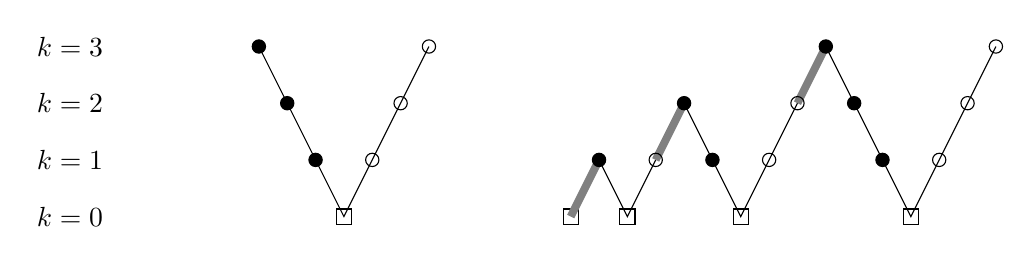
\begin{tikzpicture}[scale=1.2]
  \pgfmathsetmacro\hstep{0.3}
  \pgfmathsetmacro\vstep{0.6}
  \pgfmathsetmacro\ceps{0.08}   % size of square for coarse grid

% grid labels at left
  \node at (-2,3*\vstep) {$k=3$};
  \node at (-2,2*\vstep) {$k=2$};
  \node at (-2,\vstep) {$k=1$};
  \node at (-2,0.0) {$k=0$};

% V-cycle
  \draw[black,thin] (0.0,3*\vstep) -- (\hstep,2*\vstep) --  (2*\hstep,\vstep) -- (3*\hstep,0.0)
                    -- (4*\hstep,\vstep) -- (5*\hstep,2*\vstep) -- (6*\hstep,3*\vstep);
  \filldraw (0.0,3*\vstep) circle (2.0pt);
  \filldraw (\hstep,2*\vstep) circle (2.0pt);
  \filldraw (2*\hstep,\vstep) circle (2.0pt);
  \draw     (3*\hstep-\ceps,-\ceps) rectangle (3*\hstep+\ceps,+\ceps);
  \draw     (4*\hstep,\vstep) circle (2.0pt);
  \draw     (5*\hstep,2*\vstep) circle (2.0pt);
  \draw     (6*\hstep,3*\vstep) circle (2.0pt);

% initial coarse solve
  \pgfmathsetmacro\hoff{11*\hstep}
  \draw[shift={(\hoff,0)}]     (-\ceps,-\ceps) rectangle (+\ceps,+\ceps);
  \draw[line width=1mm,gray,shift={(\hoff,0)}] (0.0,0.0) -- (\hstep,\vstep);

% V-cycle to level 1
  \pgfmathsetmacro\hoff{12*\hstep}
  \draw[shift={(\hoff,0)},black,thin] (0.0,\vstep) -- (\hstep,0.0) -- (2*\hstep,\vstep);
  \draw[line width=1mm,gray,shift={(\hoff,0)}] (2*\hstep,\vstep) -- (3*\hstep,2*\vstep);
  \filldraw[shift={(\hoff,0)}] (0.0,\vstep) circle (2.0pt);
  \draw[shift={(\hoff,0)}]     (\hstep-\ceps,-\ceps) rectangle (\hstep+\ceps,+\ceps);
  \draw[shift={(\hoff,0)}]     (2*\hstep,\vstep) circle (2.0pt);

% V-cycle to level 2
  \pgfmathsetmacro\hoff{15*\hstep}
  \draw[shift={(\hoff,0)},black,thin] (0.0,2*\vstep) --  (\hstep,\vstep) -- (2*\hstep,0.0) -- (3*\hstep,\vstep) -- (4*\hstep,2*\vstep);
  \draw[line width=1mm,gray,shift={(\hoff,0)}] (4*\hstep,2*\vstep) -- (5*\hstep,3*\vstep);
  \filldraw[shift={(\hoff,0)}] (0.0,2*\vstep) circle (2.0pt);
  \filldraw[shift={(\hoff,0)}] (\hstep,\vstep) circle (2.0pt);
  \draw[shift={(\hoff,0)}]     (2*\hstep-\ceps,-\ceps) rectangle (2*\hstep+\ceps,+\ceps);
  \draw[shift={(\hoff,0)}]     (3*\hstep,\vstep) circle (2.0pt);
  \draw[shift={(\hoff,0)}]     (4*\hstep,2*\vstep) circle (2.0pt);

% V-cycle to finest (level 3)
  \pgfmathsetmacro\hoff{20*\hstep}
  \draw[shift={(\hoff,0)},black,thin] (0.0,3*\vstep) -- (\hstep,2*\vstep) --  (2*\hstep,\vstep) -- (3*\hstep,0.0)
                    -- (4*\hstep,\vstep) -- (5*\hstep,2*\vstep) -- (6*\hstep,3*\vstep);
  \filldraw[shift={(\hoff,0)}] (0.0,3*\vstep) circle (2.0pt);
  \filldraw[shift={(\hoff,0)}] (\hstep,2*\vstep) circle (2.0pt);
  \filldraw[shift={(\hoff,0)}] (2*\hstep,\vstep) circle (2.0pt);
  \draw[shift={(\hoff,0)}]     (3*\hstep-\ceps,-\ceps) rectangle (3*\hstep+\ceps,+\ceps);
  \draw[shift={(\hoff,0)}]     (4*\hstep,\vstep) circle (2.0pt);
  \draw[shift={(\hoff,0)}]     (5*\hstep,2*\vstep) circle (2.0pt);
  \draw[shift={(\hoff,0)}]     (6*\hstep,3*\vstep) circle (2.0pt);
\end{tikzpicture}

\caption{An FAS V-cycle (left) and F-cycle (right) on a mesh hierarchy with four levels ($K=3$).  Solid dots correspond to \texttt{down} sweeps of NGS, open circles to \texttt{up} sweeps, and squares to \textsc{coarsesolve}(). Thick grey edges represent $\hat P$.}
\label{fig:cycles}
\end{figure}

V-cycles can be done repeatedly, using the whole mesh hierarchy, to solve the original problem \eqref{weakform} to desired accuracy.  We put this in a pseudocode for clarity:

\begin{pseudo*}
\pr{fas-vcycles}(Z)\text{:} \\+
    $\ell^K[v] = \ip{g}{v}$ \\
    $w^K = 0$ \\
    for $s=1,\dots,Z$ \\+
        \pr{fas-v}(K,w^K,\ell^K) \\-
    return $w^K$
\end{pseudo*}

In \texttt{fas1.py} the option \texttt{-cycles} specifies $Z$, defaulting to $Z=1$.  As we will see in practice, five to ten V-cycles, using the default settings in \textsc{fas-vcycle} including \texttt{down} $=1$ and \texttt{up} $=1$ smoother applications, make a very effective solver on any mesh.

Next we can add a different multilevel idea.  It is based on the observation that the performance of a nonlinear equation solver usually depends critically on the quality of the initial iterate.  Indeed, choosing initial iterate $w=0$ as in \textsc{fas-vcycles} may not yield a convergent method.  However, it is easy to see in practice that coarse meshes are more forgiving with respect to the initial iterate than are finer meshes.  The additional idea is to start on the coarsest mesh in the hierarchy, where a blind guess like $w=0$ is most likely to succeed, and then work upward through the levels.  At each mesh level one computes an initial iterate by prolongation of the already-converged iterate on the next-coarser level.

The resulting algorithm is called an FAS multigrid ``F-cycle'', or, confusingly, a ``full multigrid'' (FMG) cycle \cite{BrandtLivne2011,Briggsetal2000}.  (The meaning of ``full'' is fundamentally different in ``FAS'' versus ``FMG'' terminology.)  It is shown on the right in Figure \ref{fig:cycles}.  Once the finest mesh level is reached we may do repeated V-cycles, as in the following algorithm:

\begin{pseudo*}
\pr{fas-f}(Z)\text{:} \\+
    $\ell^0[v] = \ip{g}{v}$ \\
    $w^0 = 0$ \\
    \pr{coarsesolve}(w^0,\ell^0) \\
    for $k=0,\dots,K$ \\+
        $\ell^k[v] = \ip{g}{v}$ \\
        $w^k = \hat P w^{k-1}$ \\
        if $k=K$ \\+
            for $s=1,\dots,Z$ \\+
                \pr{fas-v}(K,w^K,\ell^K) \\--
        else \\+
            \pr{fas-v}(k,w^k,\ell^k) \\--
    return $w^K$
\end{pseudo*}

FIXME F-cycle uses a better prolongation $\hat P$

In the next section we will compare three algorithms to solve the original problem \eqref{liouvillebratu} or \eqref{weakform}.  Note that each returns an iterate $w^K$ on the finest mesh:

\begin{itemize}
\item Sweeps of NGS only, defined by the following pseudocode:

\begin{pseudo*}
\pr{ngsonly}(Z)\text{:} \\+
    $\ell^K[v] = \ip{g}{v}$ \\
    $w^K = 0$ \\
    for $s=1,\dots,Z$ \\+
        \pr{ngssweep}(w^K,\ell^K) \\-
    return $w^K$
\end{pseudo*}

\item \textsc{fas-vcycles}$(Z)$ defined above.
\item \textsc{fas-f}$(Z)$ defined above.
\end{itemize}

The main conclusion of the current document can be summarized as follows:

\begin{quotation}
\emph{On any mesh of practical effective resolution, say with $m>100$ elements, the Liouville-Bratu problem \eqref{liouvillebratu} can be solved to within the discretization error of the finite element method by using \textsc{fas-f}$(2)$ or \textsc{fas-vcycles}$(10)$, regardless of $m$, up to the memory limits of the computer.  By contrast, a $Z$-value which grows rapidly with $m$ must be used with \textsc{ngsonly}$(Z)$, and $Z > 1000$ is required.  If $m>1000$ then discretization error cannot be achieved by \textsc{ngsonly}$(Z)$ in reasonable time.}
\end{quotation}

In section \ref{sec:optimal} we will carefully measure the computational work required for the three algorithms.  The work is, indeed, comparable to the quoted $Z$ values.


\section{Results: convergence}  \label{sec:convergence}

FIXME


\section{Results: optimality}  \label{sec:optimal}

FIXME; discuss work units; compare \texttt{-ngsonly}


\section{Conclusion}  \label{sec:conclusion}

FIXME


\small

\bigskip
\bibliography{fas}
\bibliographystyle{siam}

\end{document}
